\documentclass[10pt]{jarticle}
\usepackage{float}
\usepackage{adrobo_abst}
\usepackage[dvipdfmx]{graphicx}
\usepackage{amssymb,amsmath}
\usepackage{bm}
\usepackage[superscript]{cite}
\usepackage{enumerate}
\usepackage{url}
%\usepackage[absolute]{textpos}

\renewcommand\citeform[1]{(#1)}

\begin{document}
    
    \makeatletter
    \doctype{2024年度卒業論文概要}
    \title{視覚と行動のend-to-end学習により\\経路追従行動を模倣する手法の提案}{(経路選択の成功率向上を意図したネットワークの変更と実験的評価)}
    \etitle{A proposal for an imitation method of path-tracking behavior\\by end-to-end learning of vision and action}{(Experimental evaluation of network changes\\ to improve route selection success rate)}
    
    \author{21C1011\hspace{.5zw}石黒巧}
    \eauthor{Takumi ISHIGURO}
    
    \makeatother
    
    \abstract{When preparing the manuscript, read and observe carefully this sample as well as the instruction manual for the manuscript of the Transaction of Japan Society of Mechanical Engineers. This sample was prepared using MS-word. Character size of the English title is 14 pts of Times New Roman as well as sub-title. The name is 12 pts. The address of the first author and the abstract is 10 pts of Times New Roman. Character spacing of the abstract is narrowed by 0.2 pts preferably.}
    
    \keywords{Mechanical Engineering, Keywords List}
    
    \maketitle
    
    \supervisor{指導教員: 林原靖男教授}
    
    \section{緒\hspace{2zw}言}%===========================
    近年、自律移動ロボットの研究においてカメラ画像を用いたナビゲーションに関する研究が行われている。
    本研究室の岡田らはメトリックマップベースの経路追従行動を end-to-end 学習を用いて,視覚を入力として模倣することで、視覚に基づくナビゲーション手法を提案した.
    また,春山らはカメラ画像とシナリオに基づいて,任意の目的地まで自律移動するシステムを提案している.
    ここでのシナリオとは島田らが提案した,「条件」と「行動」に関する単語を組みわせて構成されている.
    この手法では,岡田らの視覚に基づいたナビゲーションに加え,カメラ画像から通路の種類を分類,シナリオによって目標方向を決定し経路を選択する機能を追加している.
    % 春山らは、島田が作成した 50 例のシナリオから 7 例を選定している。
    春山らは、島田が作成した 50 例のシナリオから 7 例を選定し,そのすべてで目的地まで到達できることを確認している。
    選定理由の1つとして、島田らが対象とするエリアから限定している。
    限定されたエリアは、ホワイエと呼ばれるスペースを一部を含むものの、壁や床の色が類似しており、一貫性のある環境といえる。
    一方、その他のエリアを含むシナリオでは、ホワイエを通り抜ける必要があることや,地面の色が異なる区域も対象としていることから,提案する手法で自律走行できないおそれがある.
    
    \section{視覚に基づいて目的地まで\\経路追従するシステム}
    本研究のベースとなる、春山らが提案した視覚に基づいて目的地まで経路追従するシステムについて述べる。
    提案されたシステムの概要を~~に示す。
    このシステムは \\
    1) シナリオを分解し,「条件」と「行動」を抽出するモジュール(以後,シナリオモジュールと呼ぶ) \\
    2) カメラ画像と目標方向を与えることで,経路を追従するモジュール(以後,経路追従モジュールと呼ぶ) \\
    3) カメラ画像から通路の特徴を分類するモジュール(以後,通路分類モジュールと呼ぶ) \\
    の3つのモジュールから構成される。
    ロボットは下記の a から d の一連の流れにより,指示された経路に沿って目的地まで自律移動する.


    (a) トポロジカルマップ上の目的地に基づき,「条件」と「行動」からなるシナリオを作成する.
        例えば,Aを目的地とする場合のシナリオは「次の角まで直進.左折.」となる.\\
    (b) シナリオモジュールにシナリオを入力し,「条件」と「行動」を抽出する.
        最初の条件と行動のセットは「次の角まで」と「直進」である.
        「直進」を目標方向として経路追従モジュールへ渡し,ロボットを制御する.
    (c) ロボットが角に近づくと,通路分類モジュールがカメラ画像に基づいて通路を「角」と判定する.
        これにより,シナリオモジュールは「次の角まで」の条件が満たされたことを確認し,次の行動「左折」へ遷移する.
    (d) 次の行動「左折」に基づいて,経路追従モジュールがロボットを制御し,角を左折する.
    
    \section{機能の改善}%===========================
    経路追従モジュールに関して,経路追従の可能性を向上させるために2点変更を加えた.
    \subsection{ネットワークの変更}
    felipeらの先行研究\cite{Codevilla2018}によると,コマンドによってモデルを分岐する形式のネットワークが春山らの先行研究で使用していた形式より経路追従の成功率が高いと報告している.
    % そのため,今回の研究ではfelipeらによって提案されたネットワークを参考に\figref{fig:branched}に示す,新たなネットワークを構築した.
    % ネットワークの入力は春山らが作成したものと同様で 64×48 の RGB画像と\tabref{tab:cmd_dir}に示す,目標方向のワンホットベクトルで,出力はヨー方向の角速度である.
    また,損失関数や活性化関数などのパラメータは春山らの手法と同様である.
    % \begin{center}
    %     \begin{figure}[!b]
    %         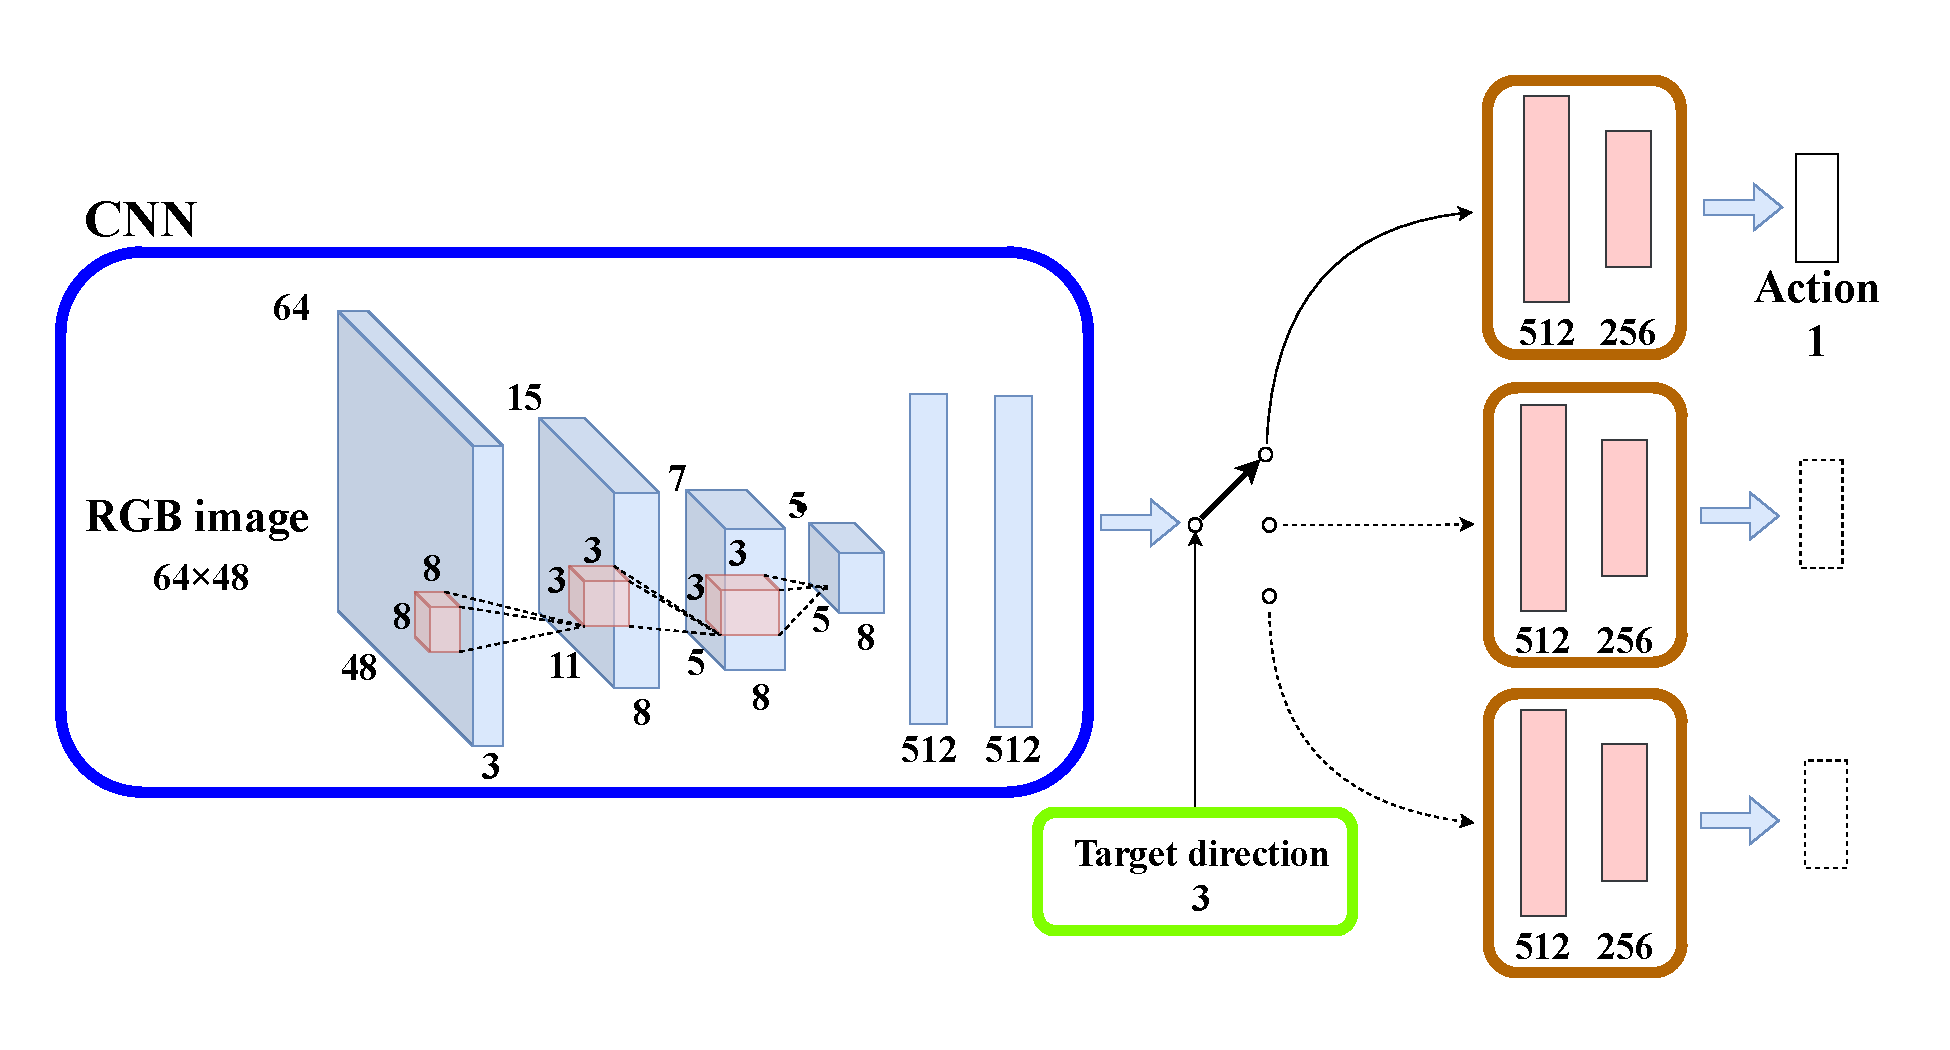
\includegraphics[width=0.45\textwidth]{./fig/branched.pdf}
    %         \caption{Branched network}
    %         \label{fig:branched}
    %     \end{figure}
    % \end{center}
    \subsection{オフライン学習の併用}
    
    \section{実験}%===========================
    実ロボットを用いて, 新たなエリアを含んだシナリオに関しても, ロボットが目的地へ到達可能であるか検証する.
    \subsection{実験装置}
    ~に示すロボットを使用する.
    また,ロボットは以下の部品で構成される\\
    1) ウェブカメラ (サンワサプライ株式会社 CMS-V43BK)\\
    2) 2D-LiDAR (北陽電機 UTM-30LX)\\
    3) PC (GALLERIA GCR2070RGF-QC-G)\\
    4) エンコーダ\\
    \subsection{実験方法}
    % 実験環境として\figref{fig:topo}に示す千葉工業大学2号館3階を用いる.

    \subsubsection{経路追従モジュールの訓練}
    % \figref{fig:route}に示すルートをオンライン学習させながら 1 周走行する.
    % データセットの収集には藤原ら\cite{fujiwara2023}が提案する手法を用いる.
    また,オンライン学習で作成したモデルに追加でオフライン学習を行う.
    オフライン学習時のデータセットにはオンライン学習の際に作成したルート 1 周分のデータを用いる.
    データセットからはオンライン学習と同様のバッチサイズ 8 でデータをランダムに取得し,epoch数は 20 とした.
   
    \subsubsection{通路分類モジュールの訓練}
    % \figref{fig:route}に示すルートをROS の navigation パッケージを使用して,経路を 1 周する.
    その際, 3 つのカメラからそれぞれ画像データを収集しながら走行する.
    学習時のパラメータとして,バッチサイズを 32 ,epoch数を 30 とした.

    \subsubsection{シナリオに基づくナビゲーション}
    2 つのモジュールを訓練後,ロボットが目的地まで到達できるか確認する.
    実験では,ロボットをシナリオのスタート地点,向きに配置し,シナリオを 1 例ずつ入力する.
    途中で壁に衝突や,経路の選択を誤ることなく自律移動し,目的地で停止した際に成功とする.

    \subsection{実験結果}
    選定したシナリオ 28 例中,24 例の成功を確認した.
    失敗した 4 例ではそれぞれ,曲がり角で左折すべきところを直進した.
    失敗の原因として,通路分類の結果の切り替わりが遅いことが考えられる.
    通路分類が遅れることで目標方向が与えるタイミングが学習時より遅くなり,左折できないことを確認した.

    \section{結\hspace{2zw}言}%===========================
    
    \vspace{5truemm}
    {\footnotesize
        \begin{thebibliography}{99}
            
            \bibitem{okada2020}
            岡田眞也 , 清岡優祐 , 上田隆一 , 林原靖男 .
            ”視覚と行動の end-to-end 学習により経路追従行動をオンラインで模倣する手法の提案 ”. 
            計測自動制御学会 SI 部門講演会 SICE-SI2020予稿集 , 
            pp.1147-1152(2020).

            \bibitem{haruyama2023}
            春山健太 , 藤原柾 , 馬場琉生 , 石黒巧 , 上田隆一 , 林原靖男 .
            "視覚と行動のend-to-end学習により経路追従行動をオンラインで模倣する手法の提案 -トポロジカルマップとシナリオに基づく経路選択機能の追加と検討-", 
            計測自動制御学会 SI 部門講演会 SICE2023 予稿集,
            pp.1B4-03(2023).
       
            \bibitem{Codevilla2018}
            F. Codevilla, M. Müller, A. López, V. Koltun, A. Dosovitskiy: 
            ``End-to-end Driving via Conditional Imitation Learning'', 
            arXiv preprint, arXiv:1710.02410 (2018), 
            \url{https://arxiv.org/abs/1710.02410}.

        \end{thebibliography}
    }
    \normalsize
    
\end{document}
